\section{The Standard Model of Particle Physics}

The Standard Model \cite{Spiesberger:2000ks} is an effective description of all known fundamental particles.  Despite this criticism, the Standard Model provides a valid framework for the description of Nature, from microscopic scales up to cosmological distances.The Standard Model consists of three components.

The first component states that the basic constituents of matter are leptons and quarks which are realized in three families of identical structure. The entire ensemble of these constituents has been identified experimentally. Table \ref{table:fermions} shows all the fermions of the Standard Model and their charges, arranged in the three families.

	\begin{figure}[tbh!]
		\begin{center}
			
			\begin{tabular}{ | c | c | c | c | c |}
				\hline
				& 1st Generation & 2 Generation & 3rd Generation & charge \\ \hline \hline
				& & & & \\
				leptons & $\left( \begin{array}{c} \nu_{e} \\ e \end{array} \right)_{L}$ & $\left( \begin{array}{c} \nu_{\mu} \\ \mu \end{array} \right)_{L}$ & $\left( \begin{array}{c} \nu_{\tau} \\ \tau \end{array} \right)_{L}$ & \begin{tabular}{@{}c@{}}weak \\ weak, electromagnetic\end{tabular} \\
				& & & & \\
				 & $e_{R}$& $\mu_{R}$& $\tau_{R}$& electromagnetic\\ 
				 & & & & \\
				 \hline
				 & & & & \\
				leptons & $\left( \begin{array}{c} u \\ d \end{array} \right)_{L}$ & $\left( \begin{array}{c} c \\ s \end{array} \right)_{L}$ & $\left( \begin{array}{c} t \\ b \end{array} \right)_{L}$ & weak, electromagnetic, strong \\
				& & & & \\
				& $u_{R}, d_{R}$& $c_{R}, s_{R}$& $t_{R}, b_{R}$& electromagnetic, strong\\
				& & & & \\ 
				\hline
				\hline
			\end{tabular}
			\caption{Fermions of the Standard Model and their charges, arranged in the three generations. Only the left-handed fermions interact weakly and are arranged in doublets. The right-handed fermions are singlets. The right-handed neutrinos are not present in this table, as they do not interact with one of the forces of the Standard Model.}
			\label{table:fermions}
		\end{center}
	\end{figure}
	
	\begin{figure}[tbh!]
		\centering
		\begin{tabular}{cc}
			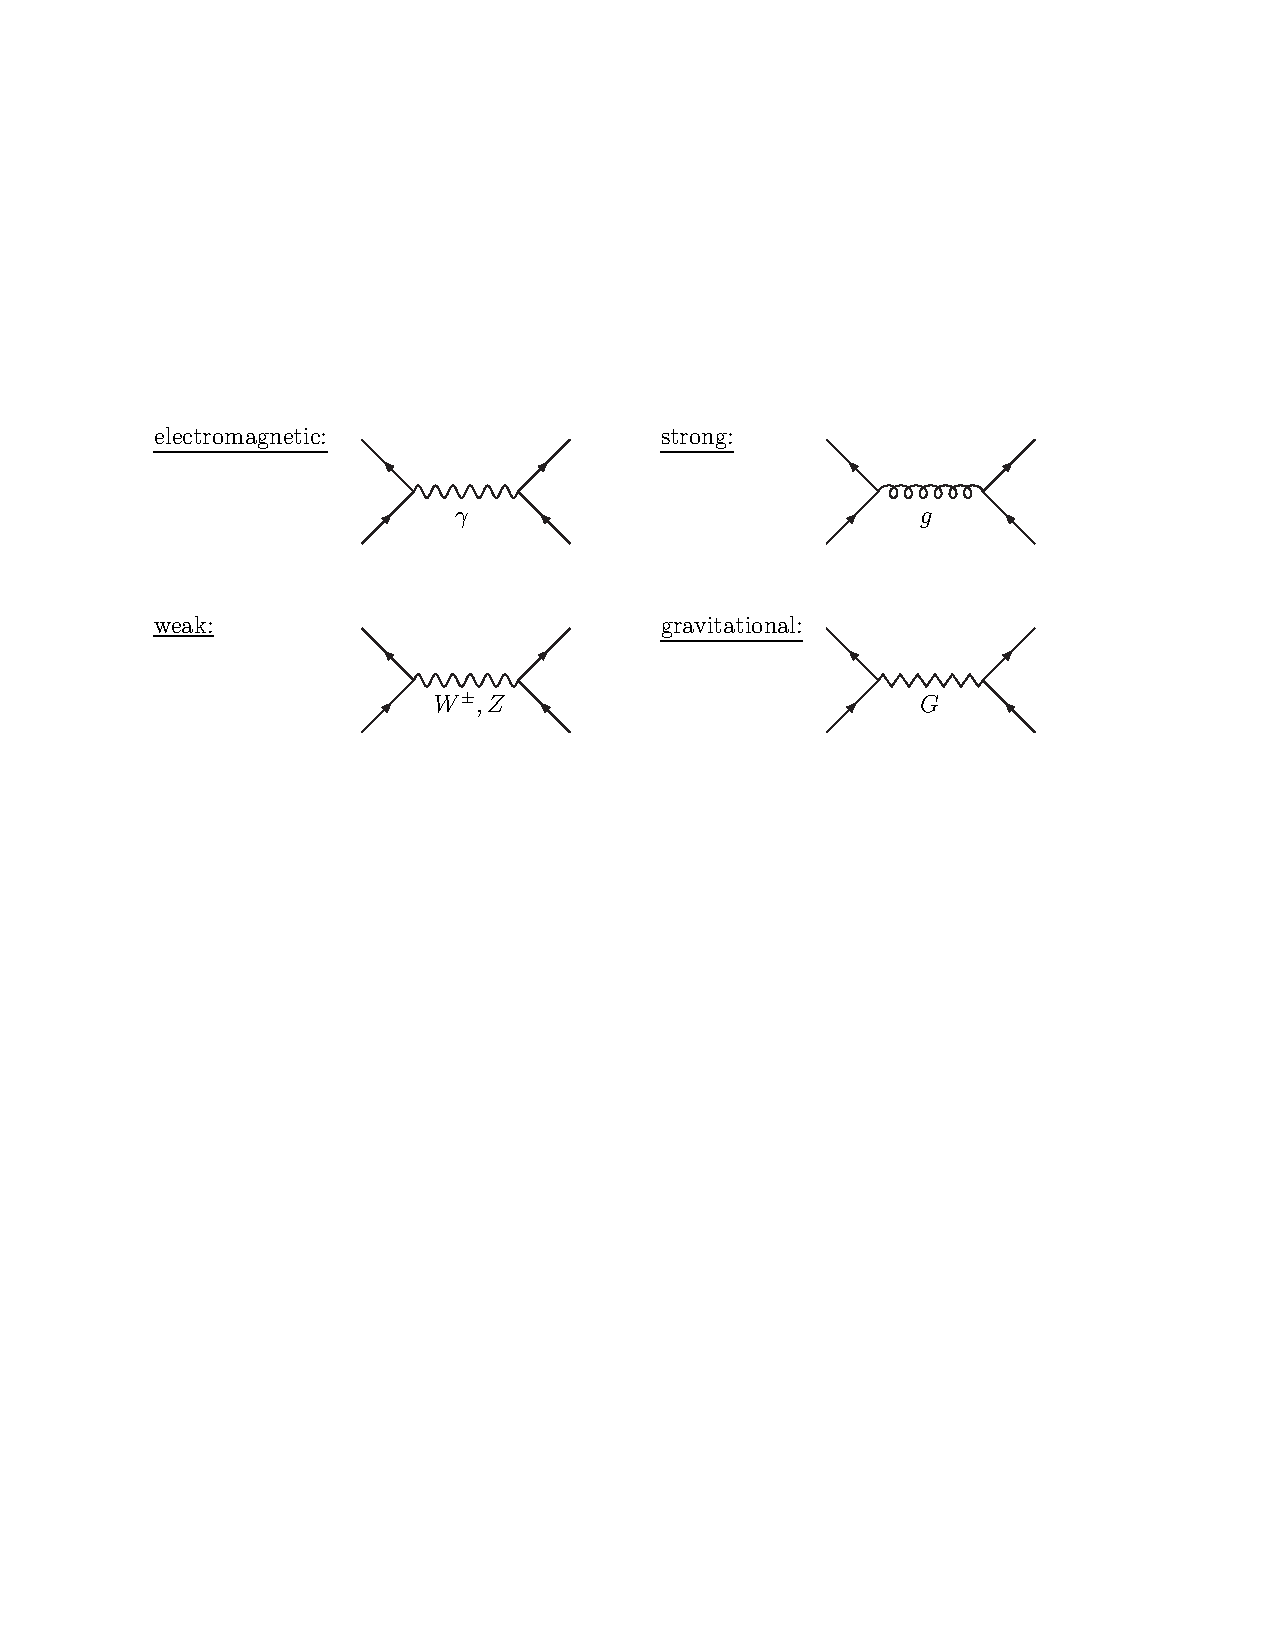
\includegraphics[width=0.75\textwidth]{theory/pics/SM_forces.pdf}
		\end{tabular}
		\caption{The four fundamental forces in nature as described by the Standard Model.}
		\label{fig:SM_forces}
	\end{figure}
	
The second component are the four different forces acting between the leptons and quarks. The electromagnetic and weak forces are unified in the Standard Model. The fields associated with these forces, as well as the fields associated with the strong force, are spin-1 fields, describing the photon \ensuremath{\gamma}, the electroweak gauge bosons \W and \Z, and the gluons g. The interactions of the force fields with the fermionic constituents of matter as well as their self-interactions are described by Abelian and non-Abelian \ensuremath{SU(3) \times SU(2) \times U(1)} gauge theories. The experimental exploration of these fundamental gauge symmetries is far advanced in the sector of lepton/quark-gauge boson interactions, yet much less is known so far from experiment about the self-interactions of the force fields. The gravitational interaction is mediated by a spin-2 field, describing the graviton G, with a character quite different from spin-1 gauge fields. The gravity sector is attached ad hoc to the other sectors of the Standard Model, not properly formulated yet as a quantum phenomenon. Figure \ref{fig:SM_forces} shows the four fundamental forces in nature as described by the Standard Model.

\begin{figure}[tbh!]
	\centering
	\begin{tabular}{cc}
		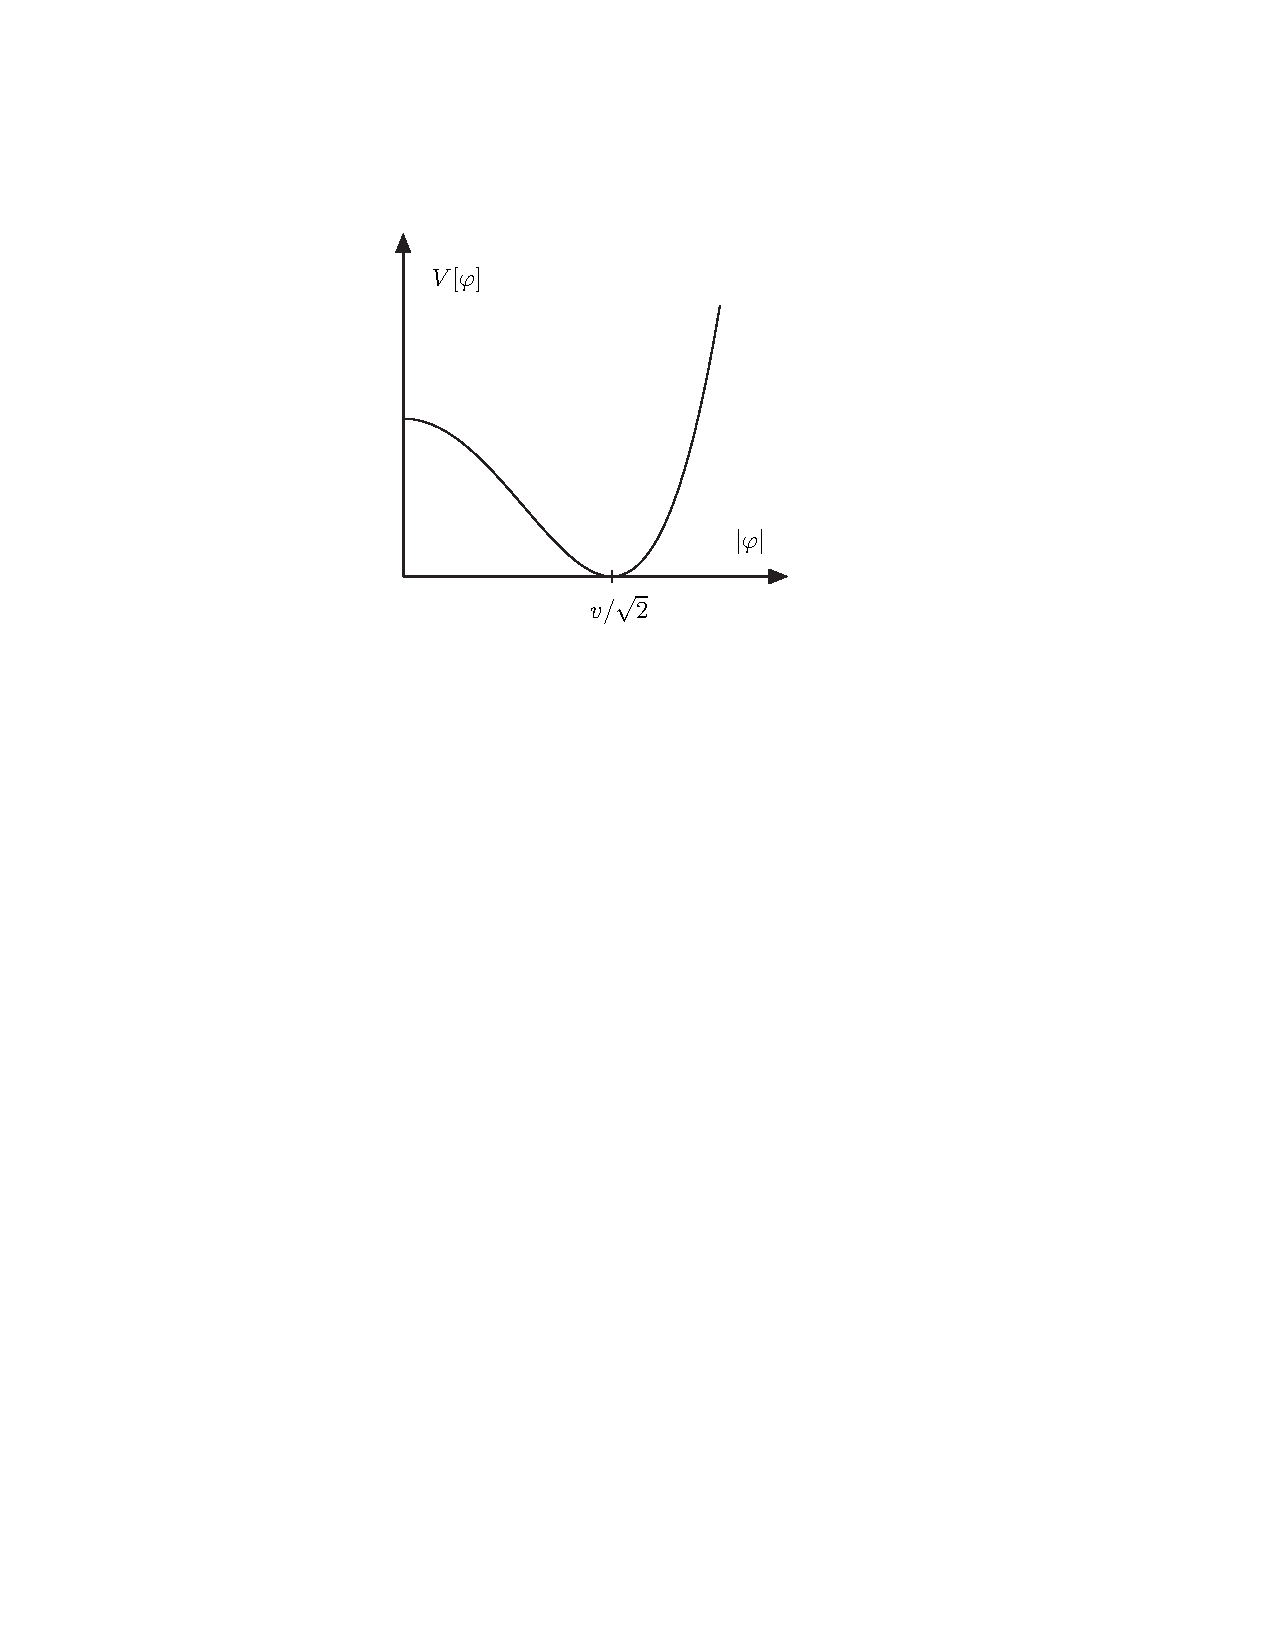
\includegraphics[width=0.75\textwidth]{theory/pics/higgs_potential.pdf}
	\end{tabular}
	\caption{The Higgs potential of the Standard Model.}
	\label{fig:higgs_potential}
\end{figure}

The third component of the Standard Model is the Higgs mechanism. In this sector of the theory, scalar fields interact with each other in such a way that the ground state acquires a non-zero field strength, breaking the electroweak symmetries spontaneously. The potential describing these self-interactions is displayed in \ref{fig:higgs_potential}. The interaction energies of electroweak gauge bosons, leptons and quarks with this field manifest themselves as non-zero masses of these particles. If this picture is correct, a scalar particle, the Higgs boson, should be observed with a mass of less than about 700 GeV, the final experimentum crucis of the Standard Model.

The the overall picture of all known Standard Model particles is shown on picture \ref{fig:SM_particles}

\begin{figure}[tbh!]
	\centering
	
	\begin{tabular}{cc}
		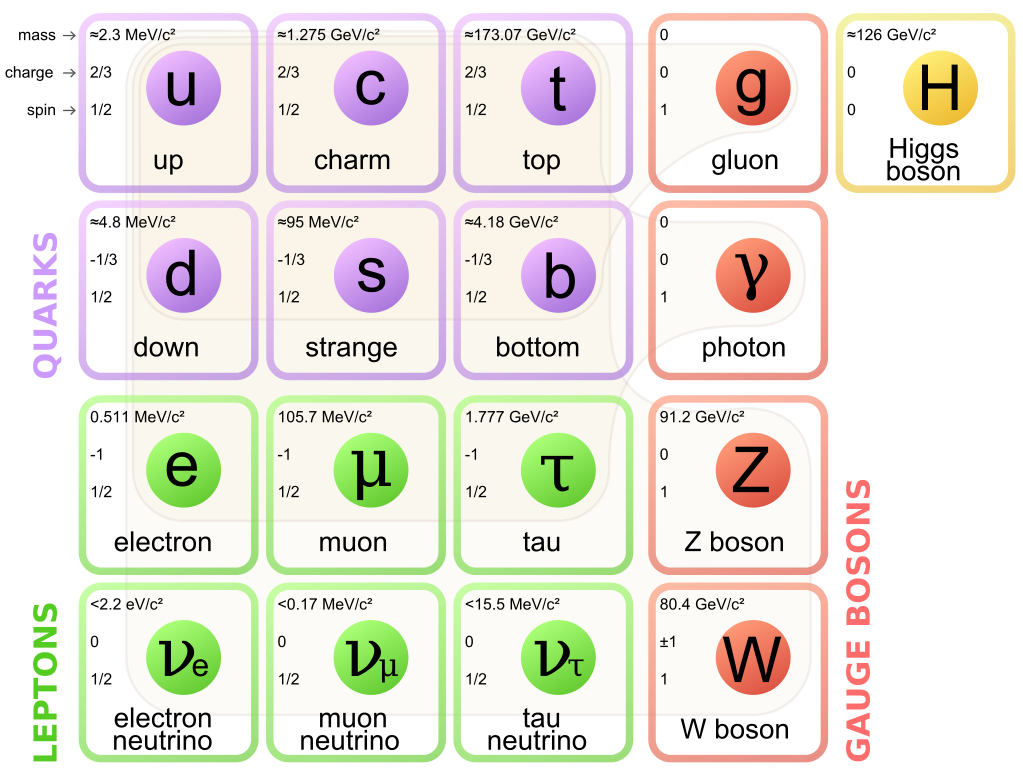
\includegraphics[width=0.75\textwidth]{theory/pics/SM_particles.png}
	\end{tabular}
	\caption{The Standard Model of elementary particles consists of  12 fundamental fermions and 4 fundamental bosons. Brown loops indicate which bosons (red) couple to which fermions (purple and green).}
	\label{fig:SM_particles}
\end{figure}

\begin{figure}[tbh!]
	\centering
	\begin{tabular}{cc}
		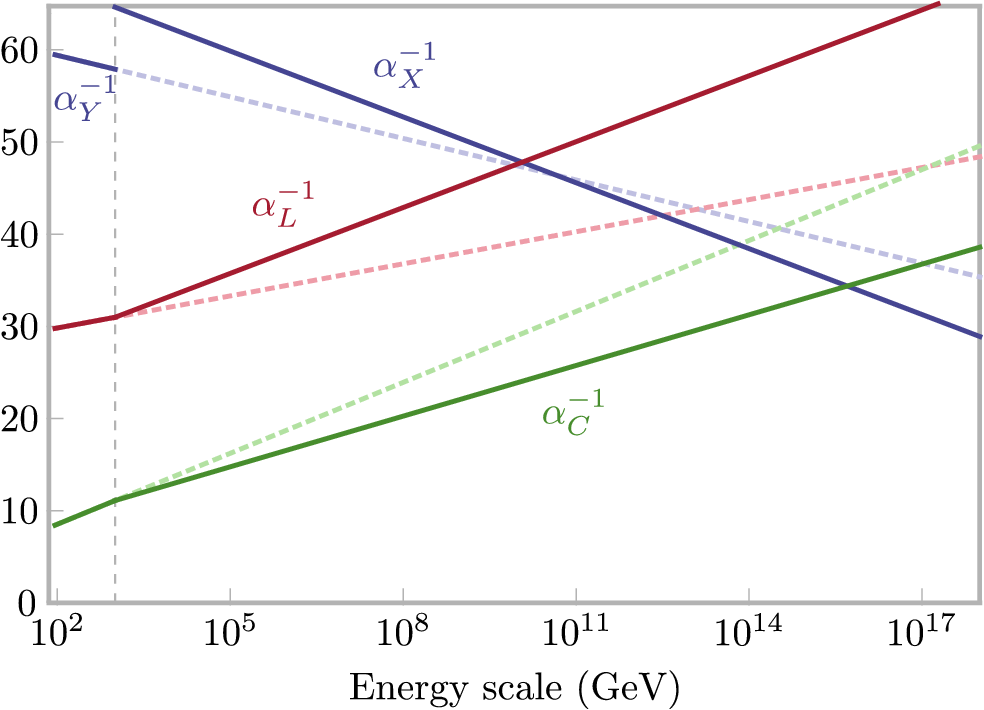
\includegraphics[width=0.75\textwidth]{theory/pics/gauge_unification.png}
	\end{tabular}
	\caption{Running of the gauge coupling constants in the SM (dashed lines) and in the model in Ref.~\cite{PhysRevD.90.013005} (solid lines). Here the $M_{331}$ scale is set to 11~TeV}
	\label{fig:gauge_unification}
\end{figure}

\clearpage

\section{Supersymmetry}

Supersymmetry is one of the most intriguing and fundamental concepts in modern theoretical particle physics. It arises naturally from the combination of the two cornerstones of 20th century physics: quantum mechanics and relativity. Supersymmetry is the unique symmetry that relates the two fundamental kinds of particles: bosons, which act as the carriers of forces, and fermions, which act as the constituents of matter. Supersymmetry transformations are in a sense like the square roots of the coordinate system transformations in special relativity, and consequently supersymmetric quantum field theories have very special, improved properties, compared to ordinary relativistic quantum field theories. If supersymmetry is realized in nature, every fermion in the SM must have a bosonic partner particle and vice versa. No such superpartner particle has been observed so far but there are more and more indications that these particles might show up at the LHC experiments.


\begin{figure}[tbh!]
	\centering
	\begin{tabular}{cc}
		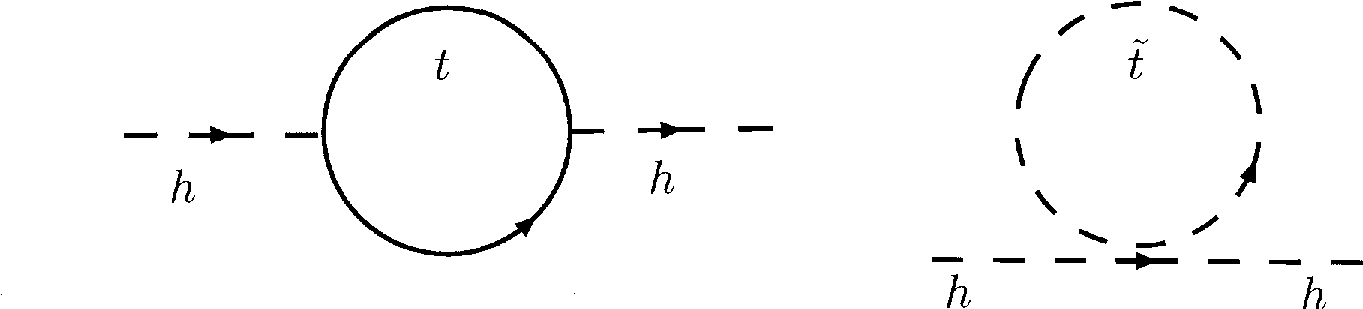
\includegraphics[width=0.75\textwidth]{theory/pics/higgs_loop.png}
	\end{tabular}
	\caption{In SUSY, the correction to Higgs mass by the top quark (L) is inherently cancelled by the contribution from the top quark's supersymmetric partner, the stop (R).}
	\label{fig:higgs_loop}
\end{figure}

\subsection{Motivations}

\subsection{The MSSM}

\begin{figure}[tbh!]
	\centering
	\begin{tabular}{cc}
		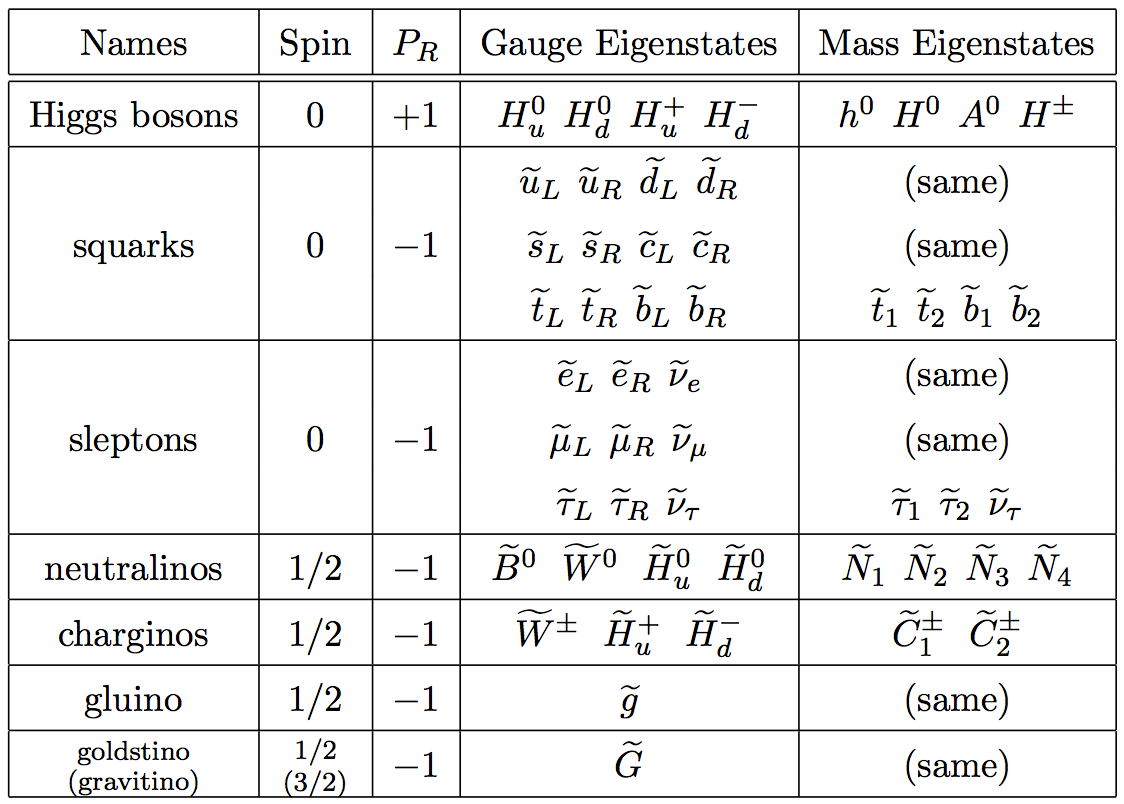
\includegraphics[width=0.75\textwidth]{theory/pics/SUSY_particles_table.png}
	\end{tabular}
	\caption{SUSY particles in MSSM~\protect\cite{Martin:1997ns}}
	\label{fig:SUSY_particles_table}
\end{figure}

\begin{figure}[tbh!]
	\centering
	\begin{tabular}{cc}
		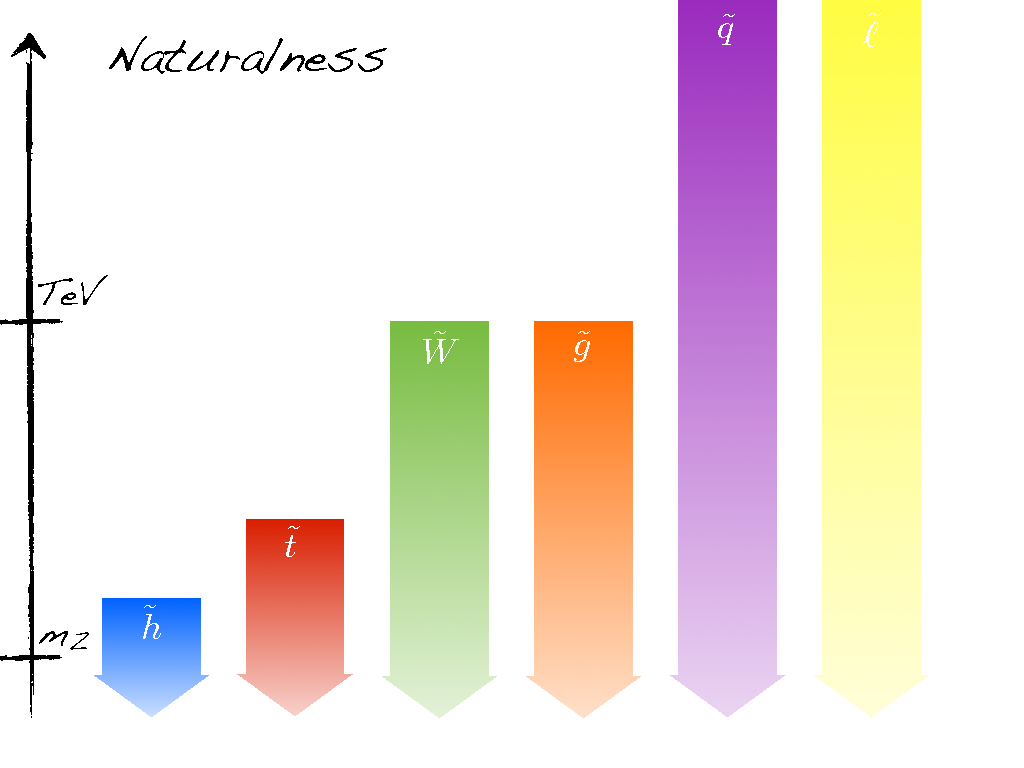
\includegraphics[width=0.75\textwidth]{theory/pics/SUSY_naturalness.png}
	\end{tabular}
	\caption{Cartoon illustration of the mass scales for various sparticles dictated solely by electroweak naturalness with sensitivity parameter $\Delta \lesssim 10$.}
	\label{fig:SUSY_naturalness}
\end{figure}




\subsection{SUSY Signatures at the LHC}
